\begin{figure*}[t]
\centering
\includegraphics[width=\textwidth]{example.pdf}
\vspace{-20pt}
\caption{Left: An example image from the CLEVR dataset, and two referring relational programs that identify the target object G. The challenge is distinguishing G from the second gray cube H. The first program identifies the target object as the ``gray object in front of the brown object'', where the brown object is the sphere F. The second program identifies the target object as the ``gray object in front of the cube''. In this case, the cube can be either B or H, but either of these choices uniquely identifies G. Right: A challenging problem instance that requires several relations to solve (especially when restricted to three free variables---i.e., $|\mathcal{Z}|=3$). The program shown is generated by our algorithm. It identifies the target object as ``the large blue cube to the left of the object to the left of a large blue rubber cube''.}
\label{fig:example}
\end{figure*}

\section{Introduction}

Incorporating symbolic reasoning with deep neural networks (DNNs) is an important challenge in machine learning. Intuitively, DNNs are promising techniques for processing perceptual information; then, symbolic reasoning should be able to operate over the outputs of the DNNs to accomplish more abstract tasks. Recent work has successfully applied this approach to question-answering tasks, showing that leveraging programmatic representations can substantially improve performance---in particular, in visual question answering, by building a programmatic representation of the question and a symbolic representation of the image, we can evaluate the question representation in the context of the image representation to compute the answer~\cite{yi2018neural,mao2019neuro,ma2019towards}.

A natural question is whether incorporating symbolic reasoning with DNNs can be useful for tasks beyond question answering. In particular, consider the problem of generating a \emph{referring expression}---i.e., an image caption that uniquely identifies a given \emph{target object} in a given image~\cite{golland2010game,kazemzadeh2014referitgame}. In contrast to visual question answering, where we translate a question to a program and then execute that program, in this case, we want to \emph{synthesize} a program identifying the target object and then translate this program into a caption.

In this paper, we take a first step towards realizing this approach. In particular, we study the problem of generating a programmatic variant of referring expressions that we call \emph{referring relational programs}. We assume we are given a symbolic representation of an image---such a representation can be easily constructed using state-of-the-art deep learning algorithms~\cite{redmon2016you,krishna2017visual,yi2018neural,mao2019neuro}---together with a target object in that image. Then, our goal is to synthesize a relational program that uniquely identifies the target object in terms of its attributes and its relations to other objects in the image. Figure~\ref{fig:example} (left) shows an example of an image from the CLEVR dataset, and two referring relational programs for object G in this image. The task for this image is challenging since G has identical attributes as H, which means that the program must use spatial relationships to distinguish them.

Our formulation of referring relational programs can take into account the uncertainty in the predictions of the DNN used to construct the symbolic representation of the image. One approach would be to use probabilistic reasoning, but doing so can be computationally intractable. Instead, we use an approach based on uncertainty sets---we construct uncertainty sets that include all DNN predictions above a certain probability threshold, and require that the referring relational program uniquely identify the target object for \emph{all} possible configurations in these uncertainty sets.

Based on this formulation, we propose an algorithm for synthesizing referring relational programs
%\aws{typo -- not sure how sentence should end}
given the symbolic representation of the image. Fundamentally, program synthesis is a combinatorial search problem. The objective is to search over the space of possible programs to find one that achieves the given goal---in our case, find a relational program that uniquely identifies the target object when evaluated against the symbolic representation of the image.

To account for the combinatorial size of the search space, our synthesis algorithm builds on recent techniques for speeding up program synthesis. First, it leverages \emph{execution-guided synthesis}~\cite{chen2018execution}, where deep learning is used to guide the search over the space of programs. This approach formulates the search problem as a Markov decision process, where actions correspond to decisions about which statements to include in the program, and states correspond to the intermediate program state obtained by incrementally evaluating the program generated so far. Then, it uses deep reinforcement learning to solve the synthesis problem. In particular, we use deep $Q$-learning, where the $Q$-network is a graph convolutional network (GCN) that takes as input a graph encoding of the program state; then, the $Q$-value for each action is evaluated based on local representations, avoiding the use of a lossy global representation.

Second, we leverage \emph{hierarchical synthesis}~\citep{nye2019learning}, where the neurosymbolic synthesizer is combined with a faster but unguided enumerative synthesizer---intuitively, the neurosymbolic synthesizer generates the majority of the program. Then, the enumerative synthesizer fills in the remainder of the program, which tends to be a smaller but more challenging search problem. Finally, we use a simple \emph{meta-learning} approach~\cite{si2018learning}, where the $Q$-network is pretrained on a benchmark of training synthesis tasks; this $Q$-network is used to initialize the $Q$-networks for solving future synthesis tasks.

We evaluate our approach on the CLEVR dataset~\cite{johnson2017clevr}, a synthetic dataset of objects with different attributes and spatial relationships. Our goal is to generate a relational program that identifies one of the objects in the scene. We consider both synthetic examples where the ground truth scene graph is known, as well as cases where the scene graph is predicted using a convolutional neural network (CNN) and may be prone to error.

We leverage control over the data generation process to generate problem instances that are particularly challenging---i.e., where there are multiple objects with the same attributes in each scene. By doing so, a valid relational referring program must include
%\aws{too much "leverage"}
complex spatial relationships to successfully identify the target object. We demonstrate how our approach outperforms several baselines, including a state-of-the-art program synthesizer~\cite{si2018learning}.

%Problem formulation (**) \\ 
%Motivating example \\
%Defining the language \\ 
%Keep it more intuitive rather than formal notation \\
%Don't need to define the syntax too much. Give examples. 

%1. Overview describe of problem \\
%2. Reference through out text \\
%3. Define language & environment  \\

%Formulation as an RL problem, action, state, transition, reward, algorithm.  \\
%Spec: Goal - shortest path program uniquely identify the object. Set of the object to the scene that the variable could bind to. \\ 

%The experiment is of higher priority. 
%Tip for Latex: Macro for Notation. \\

\textbf{Related work.}
%
There has been a great deal of recent interest in leveraging program synthesis to improve machine learning---e.g., to classify images based on their parts~\cite{lake2015human}, to infer the structure of images~\cite{ellis2015unsupervised,ellis2018learning,pu2018selecting}, to perform procedural tasks over images~\cite{gaunt2017differentiable,valkov2018houdini}, to generate images with programmatic structure~\cite{young2019learning}, and interpretable and robust reinforcement learning~\cite{verma2018programmatically,bastani2018verifiable,verma2019imitation,jothimurugan2019composable,inala2020synthesizing}. These techniques demonstrate how incorporating program synthesis into machine learning tasks can improve performance on tasks that involve programmatic or symbolic reasoning.

Most closely related, there has been interest in leveraging programmatic reasoning in the domain of visual question answering~\cite{mao2019neuro,ma2019towards}. These approaches translate the question into a program using semantic parsing, and translate the image into a symbolic representation (e.g., a scene graph encoding the object attributes and relationships); then, they execute the program in the context of the symbolic representation as input to produce the answer to the given question.

Whereas visual question answering corresponds to \emph{executing} a program in the context of the scene graph, our key insight is that generating a referring expression corresponds to \emph{synthesizing} a program that, when executed in the context of the scene graph, produces the given target object.

There has been work on incorporating logical reasoning into deep neural networks to perform reasoning tasks such as sorting and shortest path~\cite{dong2019neural} or solving Sudoku problems~\cite{wang2019satnet}, including work incorporating relational reasoning into deep neural networks to improve question answering~\cite{santoro2017simple} and planning~\cite{santoro2018relational}, as well as general frameworks incorporating relational programs with probabilistic inference~\cite{de2007problog} or deep learning~\cite{cohen2018tensorlog,manhaeve2018deepproblog}. In contrast, our goal is to \emph{generate} relational programs to achieve some goal.

There has been work on synthesizing relational programs~\cite{albarghouthi2017constraint,si2018syntax,raghothaman2019provenance,si2019synthesizing}, though this work focuses on relational programs with different structure than ours. In particular, they typically assume the space of possible rules is not too large, and the goal is to find the right combination of rules; in contrast, our goal is to find a single rule in a combinatorially large search space of rules. There has also been work on using machine learning to speed up synthesis~\cite{menon2013machine,balog2017deepcoder,parisotto2017neuro,bunel2018leveraging,feng2018program,ellis2018dreamcoder}; which we leverage in our algorithm.

\section{Referring Relational Programs}

\textbf{Scene graph representation of images.}
%
%\aws{do we need a complicated n-ary formlalization -- my understanding is all predicates are 1-2-ary}
We represent images via \emph{scene graphs} $G \in \graphs$. Vertices in $G$ are objects in the image, and edges encode relations between objects. Unary relations represent attributes such as color and shape, and binary relations capture spatial information between objects---above, left, right, and the like. Abstractly, we think of $G$ as a set of relations over objects:
\begin{align*}
G=\set{\rho_i(o^i_1, \dots, o^i_{n_i})}_{i=1}^n,
\end{align*}
where $\rho_i\in\mathcal{R}$. Relations $\rho(o_1,...,o_n)$ can be certain, uncertain, or absent. Certain are guaranteed to be in the graph, absent relations are guaranteed to not be in the graph, and uncertain relations may or may not be in the graph. We represent this decomposition by writing $G = G_+ \sqcup G_?$ as the \emph{disjoint union} of the certain relations $G_+$ and the uncertain relations $G_?$; absent relations are omitted.

\textbf{Relational programs.}
%
Our search space consists of \emph{relational programs}, which we view as sets of relations over variables. More precisely, let $\vars$ be a finite set of variables, with $\tvar \in \vars$ a \emph{target variable} representing the object being referred to. A relational program has the form:
\begin{align*}
P = \bigwedge_{i=1}^m\rho_i(z^i_1,...,z^i_{n_i}).
\end{align*}
%where \emph{at least} one $z_j^i$ is the target variable $\tvar$.
A \emph{valuation} $v \in \valuations$ is a function $v : \vars \to \objects$ that maps each variable to an object in the scene. Given a valuation, we can \emph{ground} the variables in a program using $\interp{\cdot}$:
%\aws{we might want to say what [[]] means for an ML audience}
\footnote{We use the notation $\interp{P}_v$ to denote the \emph{semantics} of a program $P$---i.e., the output obtained by evaluating $P$. In our case, $P$ evaluates into a logical formula over objects, which can be interpretered as a function mapping scene graphs to true/false.} 
\begin{align*}
\interp{P}_v=\bigwedge_{i=1}^m\rho_i(v(z^i_1),...,v(z^i_{n_i}))
\end{align*}
We will equivalently interpret $\interp{P}_v$ as the set of concrete relationships in the conjunction---i.e.,
\begin{align*}
\interp{P}_v&=\left\{\rho_i(v(z^i_1),...,v(z^i_{n_i}))\right\}_{i=1}^m
\end{align*}
In this case, the grounding $\interp{\cdot}$ converts $P$ into a set of predicates over objects. Then we can treat $\interp{P}_v : \graphs \to \bool$, where $\bool=\{\text{true},\text{false}\}$, as a Boolean function over scene graphs defined so that
\begin{align*}
\interp{P}_v(G)=(\interp{P}_v \subseteq G),
\end{align*}
i.e., $\interp{P}_v(G)$ is true if and only if all of the relationships in $\interp{P}_v$ are also contained in $G$.
\begin{definition}
\rm
A valuation $v\in\mathcal{V}$ is \emph{valid} for relational program $P$ and scene graph $G$ iff $\interp{P}_v(G)=\text{true}$.
\end{definition}
We denote the set of all valid valuations for $P$ in $G$ by
\begin{align*}
\interp{P}_G = \set{v \in \valuations \mid \interp{P}_v(G)}.
\end{align*}

\textbf{Referring relational programs.}
%
Our goal is to generate a relational program that satisfies the properties of a referring expression \cite{golland2010game,kazemzadeh2014referitgame}. Given a scene and an object $\tobj$ in that scene, a referring expression is a natural language caption that uniquely identifies $\tobj$. Figure~\ref{fig:example} shows an example of an image together with referring relational programs that identify the target object in that image, and Figure~\ref{fig:graph} shows an example of a scene graph (ignoring the gray variable nodes).

%\aws{i think we should prominently emphasize that graphs can be easily generated by a CNN -- here and in the intro as well}
We study a \emph{symbolic variant} of this problem---i.e., (i) we assume the image is given as a scene graph $G$ (e.g., these can be constructed using deep learning~\cite{redmon2016you,krishna2017visual,yi2018neural,mao2019neuro}), and (ii) our referring expressions are relational programs that uniquely identify $\tobj$. More precisely, given a scene graph $G$ and an object $\tobj$ in $G$, we want to construct a relational program $P$ such that $\tvar$ \emph{must} refer to $\tobj$ in the context of $G$.

\begin{definition}\label{def:refexpr}
\rm
Given scene graph $G$ and target object $\tobj$ in $G$, $P$ is a \emph{referring relational program} for $\tobj$ in $G$ if (i) $\interp{P}_{G_+}\neq\varnothing$, and (ii) for all $v \in \interp{P}_G$, $v(\tvar) = \tobj$.
\end{definition}

Intuitively, a referring relational program must (i) have at least one certain interpretation, and (ii) all interpretations must refer to the target object, \emph{regardless of the value of uncertain relations}. In the rest of this paper, we assume $\tobj$ is encoded in $G$ via a unary \emph{target} relation, and use the predicate $\rrp{G}{P}$ to indicate $P$ is a referring relational program for the encoded $\tobj$ in $G$.

\begin{algorithm}[t]
\begin{algorithmic}
\FUNCTION{SynthesizeProgram($G$)}
\STATE Initialize $Q$-network $Q_{\theta}$ with pretrained parameters $\theta^0$
\FOR{$i\in\{1,...,N\}$}
\STATE Sample program $P$ of length $M$ according to $Q_{\theta}$
\IF{$\rrp{G}{P}$}
\STATE \textbf{return} $P$
\ENDIF
\STATE Update $Q_{\theta}$ using deep $Q$ learning
\ENDFOR
\STATE Get best length $M-K$ program $P^0$ according to $Q_{\theta}$
\FOR{Programs $P$ of length $K$}
\IF{$\rrp{G}{P^0\wedge P}$}
\STATE \textbf{return} $P^0\wedge P$
\ENDIF
\ENDFOR
\STATE \textbf{return} $\varnothing$
\ENDFUNCTION
\end{algorithmic}
\caption{Our algorithm for synthesizing referring relational programs. Hyperparameters are $N,M,K\in\mathbb{N}$.}
\label{alg:synth}
\end{algorithm}
\section{Program Synthesis Algorithm}

\begin{figure}[t]
\centering
\includesvg[width=0.7\columnwidth]{graph.svg}
\caption{Example of a graph encoding of a state. Variables are shown in gray and objects are shown in purple. Binary relationships are shown in red (for a vertex $\rho$) and pink (for a vertex $(i,\rho_i)$). Unary relationships are shown in yellow; these relationships only have a single object, so we do not need a separate vertex for each relationship in $(i,\rho_i)$. The target relationship is shown in blue.}
\label{fig:graph}
\end{figure}

\begin{figure*}[t]
\centering
\includegraphics[width=\textwidth]{overview.pdf}
\caption{Example rollout according to our MDP. The input is a symbolic representation of the image as a graph. The states encode possible assignments of variables to objects in the scene; these are represented as graphs such as the one shown in Figure~\ref{fig:graph}. The actions are clauses $\rho(z_1,...,z_n)$; an action is chosen according to the $Q$-values predicted by the GNN $Q$-network. The interpreter, which serves as the ``environment'', removes the variables assignments that are no longer permitted by the newly chosen clause.}
\label{fig:mdp}
\end{figure*}

Next, we describe our algorithm that, given a scene graph $G$, synthesizes a referring relational program $P$ for $G$. At a high level, we formulate the synthesis problem as a Markov decision process (MDP). We then use reinforcement learning to learn a good policy $\pi$ for this MDP on a training benchmark. Then, given a new test graph $G$, we continue to fine-tune $\pi$ holding $G$ fixed, and return once we find a referring relational program $P$ for $G$. Our algorithm is summarized in Algorithm~\ref{alg:synth}.

\textbf{Formulation as an MDP.}
%
We begin by describing how to formulate the problem of synthesizing a referring relational program as a Markov decision process (MDP); Figure~\ref{fig:mdp} visualizes our MDP. Intuitively, since we want the MDP to encode a search over relational programs, one approach would be to choose the states to be relational programs $P$ and the actions to be predicates $\rho(z_1,...,z_n)$; then, taking such an action in state $P$ transitions the system to
\begin{align*}
P'=P\wedge\rho(z_1,...,z_n)
\end{align*}
While this approach is possible, the states are not very informative since they do not encode any information about the semantics of relational programs. Intuitively, a policy for this MDP would have to internally construct an interpreter for relational programs to achieve good performance.

Instead, we build on an approach known as \emph{execution-guided synthesis}~\cite{chen2018execution}, where the states are the outputs produced by executing programs $P$. Intuitively, our goal is to compute a program $P$ such that all consistent valuations uniquely identify the target object---i.e., $v(\tvar)=\tobj$. Thus, given a graph $G \in \graphs$ for the current image (which is fixed for a rollout),
we consider the output of $P$ to be the set of valuations $v \in \valuations$ that are consistent with $G$.

In particular, the states $s\in S$ in our MDP are $s=(G,V)$, where $G$ is a scene graph and $V \subseteq \valuations$ is a subset of valuations. Given a graph $G$, the initial state is $s_0=(G,\valuations)$; this choice corresponds to the empty program $P_0=\text{true}$ (so $\interp{P_0}_G = \valuations$). Next, the actions $a\in A$ in our MDP are $a=(\rho,z_1,...,z_n)\in\mathcal{R}\times\mathcal{Z}^*$,%
\footnote{Here, $*$ denotes the Kleene star---i.e., a list of variables with variable but finite length.} where $\rho$ is an $n$-ary relationship. Then, the (deterministic) transitions are
\begin{align*}
(G,V')&=T((G,V),(\rho,z_1,...,z_n)) \\
V'&=\{v\in V\mid\llbracket\rho(z_1,...,z_n)\rrbracket_v(G)\}.
\end{align*}
That is, $V'$ is the set of all valuations that are consistent with $G$ given the additional predicate $\rho(z_1,...,z_n)$. Finally, we use a sparse reward function
\begin{align*}
R((G,V))=
\begin{cases}
1&\text{if}~\forall v \in V .\ v(\tvar) = \tobj \\
0&\text{otherwise}.
\end{cases}
\end{align*}
In particular, suppose we take a sequence of actions
\begin{align*}
(\rho_1,z^1_1,...,z^1_{n_1}),...,(\rho_m,z^m_1,...,z^m_{n_m}).
\end{align*}
Then, letting $P$ be the relational program
\begin{align*}
P=\bigwedge_{i=1}^m\rho_i(z^i_1,...,z^i_{n_m}),
\end{align*}
the state $V$ after taking these actions equals is
\begin{align*}
V=\{v\in\mathcal{V}\mid\llbracket P\rrbracket_v(G)\}=\llbracket P\rrbracket_G.
\end{align*}
Thus, $R((G,V))=1$ if and only if the program $P$ corresponding to the sequence of actions taken is a referring relational program for $G$. Thus, a policy that achieves good reward on this MDP should quickly identify a valid referring relational program for a given graph $G$.

To handle uncertain relationships, we keep track of both certain and uncertain relationships---i.e., the initial state is $s_0=(G,\mathcal{V},\varnothing)$, and the transitions are
\begin{align*}
(G,V_+',V_?')=T((G,V),(\rho,z_1,...,z_n))
\end{align*}
where
\begin{align*}
V_+' =& \set{v \in V_+ \mid \interp{\rho(z_1,...,z_n)}_v(G_+)} \\
V_?' =& \set{v \in V_? \mid \interp{\rho(z_1,...,z_n)}_v(G)} \\
     &\hspace{0.1in}\cup \set{v \in V_+ \mid \interp{\rho(z_1,...,z_n)}_v(G_?)}.
\end{align*}
Finally, the rewards are as before---i.e.,
\begin{align*}
R((G,V_+,V_?))=
\begin{cases}
1&\text{if}~\forall v \in V_+ \cup V_? .\ v(\tvar) = \tobj \\
0&\text{otherwise}.
\end{cases}
\end{align*}

\textbf{Reinforcement learning.}
%
We use the deep $Q$-learning algorithm with a replay buffer to perform reinforcement learning---surprisingly, we found this approach outperformed policy gradient and actor-critic approaches. Intuitively, we believe it works well since the states in our formulation capture a lot of information about the progress of the policy. Given the deep $Q$-network $Q_{\theta}(s,a)$, the corresponding policy $\pi$ is to use $Q_{\theta}(s,a)$ with $\epsilon$-greedy exploration---i.e., $\pi(s)=\operatorname*{\arg\max}_{a\in A}Q_{\theta}(s,a)$ with probability $1-\epsilon$, and $\pi(s)\sim\text{Uniform}(A)$ with probability $\epsilon$.

\begin{figure*}[t]
\centering
\includegraphics[width=0.95\textwidth]{Qnetwork.pdf}
\vspace{-10pt}
\caption{Our $Q$-network architecture. It takes as input an encoding of the state as a graph, and produces a vector embedding for each node using a GCN. Then, it predicts $Q(s,a)$ based on the vector embeddings for the nodes in the graph relevant to the action $a$.} 
\label{fig:mdp}
\end{figure*}

\textbf{State encoding.}
%
A key challenge is designing a neural network architecture for predicting $Q_{\theta}(s,a)$. Our approach is based on encoding $s=(G,V)$ as a graph data structure, and then choosing $Q_{\theta}(s,a)$ to be a graph neural network (GNN). Our graph encoding of $(G,V)$ has three main kinds of vertices: (i) objects $o$ in $G$, (ii) relationships $\rho\in\mathcal{R}$, and (iii) variables $z\in\mathcal{Z}$, as well as a few auxiliary kinds of vertices to support the graph encoding. In Figure~\ref{fig:graph}, we show an example of a graph encoding of a state in our MDP.

First, each object $o$ is represented by exactly one vertex in the graph; each relationship $\rho\in\mathcal{R}$ is represented by exactly one vertex in the graph; and each variable $z\in\mathcal{Z}$ is represented by exactly one vertex in the graph.

Second, for each relationship $\rho_i(o_{i,1},...,o_{i,n_i})\in G$, we introduce $n+1$ new vertices $\{(i,\rho_i),(i,1),...,(i,n_i)\}$ into the graph, along with the edges
\begin{align*}
(i,\rho_i)\to(i,1)\to o_1,...,(i,\rho_i)\to(i,n_i)\to o_{n_i}
\end{align*}
as well as the edge $\rho_i\to(i,\rho_i)$. This approach serves two purposes. The first purpose is that the intermediate vertex $(i,\rho_i)$ distinguishes different relationships in $G$ with the same type $\rho_i\in\mathcal{R}$. In addition, the edges $\rho_i\to(i,\rho_i)$ connects all relationship of the same type, which allows information to flow between these parts of the graph---for example, these edges could help the GNN count how many occurrences of the relationship ``red'' are in $G$. The second purpose is that the intermediate vertices $(i,j)$ preserve information about the ordering of the objects in the relationship---e.g., in $\text{front}(o,o')$, the edge $(i,0)\to o$ indicates that $o$ is in front, and $(i,1)\to o'$ indicates that $o'$ is behind.

Third, to encode the valuations $v\in V$, we include the following edges in the graph:
\begin{align*}
\bigcup_{v\in V}\{z\to v(z)\mid z\in\mathcal{Z}\}.
\end{align*}
Intuitively, these edges capture all possible assignments of objects $o$ to variables $z$ that are allowed by $V$. For instance, in the initial state $S_0=(G,\mathcal{V})$, these edges are $z\to o$ for every $z\in\mathcal{Z}$ and $o$ in $G$. This encoding loses information about $V$, since an assignment $o$ to $z$ may only be allowed for a subset of $v\in V$. However, $V$ is combinatorial in size, so encoding the entire structure of $V$ yields too large a graph.

To ensure that information can flow both ways, all edges in our encoding described above are bidirectional.

Finally, for settings $G=(G_+,G_?)$ where we consider uncertain relationships, we encode whether the relationship is certain as an edge type $\rho\xrightarrow{+}(i,\rho_i)$ for certain relationships in $G_+$ and $\rho\xrightarrow{?}(i,\rho_i)$ for uncertain relationships in $G_?$. Similarly, we use $z\xrightarrow{+}v(z)$ for certain valuations $v\in V_+$ and $z\xrightarrow{?}v(z)$ for uncertain valuations $v\in V_?$.

\textbf{Neural network architecture.}
%
As mentioned above, $Q_{\theta}(s,a)$ is based on a graph convolutional network (GCN)~\cite{kipf2016semi}. We use $\psi(s)$ to denote the graph encoding of $s=(G,V)$ described above, where in addition each node is represented by a fixed embedding vector depending on its node name. The relationship vertices $\rho$ and $(i,\rho_i)$ have an embedding vector $x_{\rho}$. The positional vertices $(i,j)$ encoding object ordering use an single embedding $x_{\rho_i,j}$ specific to both the corresponding relationship $\rho_i$ and the object position $j$ within the relationship.

Now, $Q_{\theta}$ applies a sequence of graph convolutions to $\psi(s)$:
\begin{align*}
\psi^{(0)}&=\psi(s) \\
\psi^{(t+1)}&=f_{\theta}^{(t)}(\psi^{(t)})\hspace{0.1in}(\forall t\in\{0,1,...,m-1\}.
\end{align*}
Each $\psi^{(t)}$ has the same graph structure as $\psi(s)$, but the embedding vectors $x_k^{(t)}$ associated with each vertex $k$ are different (i.e., computed as a function of the embeddings in the previous layer and of the GCN parameters).

Finally, at the output layer, $Q_{\theta}$ decodes the $Q$-values for each action $\rho(z_1,...,z_n)$ based on the embedding vectors of the corresponding vertices $\rho,z_1,...,z_n$:
\begin{align*}
Q_{\theta}(s,\rho(z_1,...,z_n))=g_{\theta}(x_{\rho}^{(m)},x_{z_1}^{(m)},...,x_{z_n}^{(m)})
\end{align*}
The architecture of $g_{\theta}$ can be any aggregation method from vertex level to action level. Two example strategies are LSTM structure and concatenation. 

\textbf{Hierarchical synthesis.}
%
We adopt an approach based on \emph{hierarchical synthesis}~\cite{nye2019learning}. The idea is to combine a neurosymbolic synthesizer with a traditional one based on enumerative search. Intuitively, the neurosymbolic synthesizer can determine the majority of the program, after which the enumerative synthesizer can be used to complete the program into one that satisfies $\phi_G(P)$.

More precisely, in the first phase, we run the neurosymbolic synthesizer for a fixed number $N$ of steps. At each step in this phase, we generate a program $P$ of length $M$; if we find one that satisfies $\phi_G(P)$, then we return it. Otherwise, we continue to the second phase. In this phase, we begin by constructing the best program $P^0$ of length $M-K$ according to $Q_{\theta}$ (i.e., use zero exploration $\epsilon=0$), where $K\in\mathbb{N}$ is a hyperparameter of our algorithm. Then, we perform an exhaustive search over programs $P$ of length $K$, checking if the combined program $P'=P^0\wedge P$ satisfies $\phi_G(P')$. If we find such a program, then we return it. Finally, we return $\varnothing$ if we do not find a valid program, indicating failure.  

\textbf{Meta-learning.}
%
Finally, the algorithm we have described so far is for synthesizing a single referring relational program from scratch for a given scene graph $G$. We use a simple meta-learning approach where we pretrain $Q_{\theta}$ on a training benchmark of similar synthesis problems. In particular, we assume given a training set $\mathcal{G}_{\text{train}}\subseteq\mathcal{G}$ of scene graphs; then, we use deep $Q$-learning to train a neural network $Q_{\theta^0}$ that achieves high reward on average for random 
\begin{align*}
\theta^0=\operatorname*{\arg\max}_{\theta}\mathop{\mathbb{E}}_{G\sim\text{Uniform}(\mathcal{G}_{\text{train}})} \;[J(\theta;G)],
\end{align*}
where $J(\theta;G)$ is the standard $Q$-learning objective for the MDP constructed for scene graph $G$.

\textbf{Overall algorithm.}
%
Our overall algorithm is summarized in Algorithm~\ref{alg:synth}. It takes as input a scene graph $G$, and outputs a relational referring program $P$ (i.e., that satisfies $\phi_G(P)$), or $\varnothing$ if it fails to find such a program. The first step initializes $Q_{\theta}$ with the pretrained parameters $\theta^0$. Then, the first phase uses deep $Q$-learning to tune $\theta$ based on programs $P$ of length $M$ sampled from the MDP for $G$. If no valid program is found, then it proceeds to the second phase, where it performs an exhaustive enumerative search over programs $P^0\wedge P$, where $P^0$ is the optimal program of length $M-K$ according to $Q_{\theta}$. If again no valid program is found, then it returns $\varnothing$ to indicate failure.

\section{Experiments}

\begin{figure*}[t]
\centering
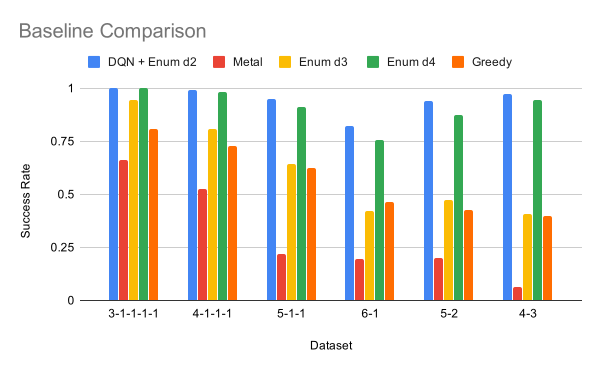
\includegraphics[width=0.4\textwidth]{baselines.pdf}
\hspace{0.5in}
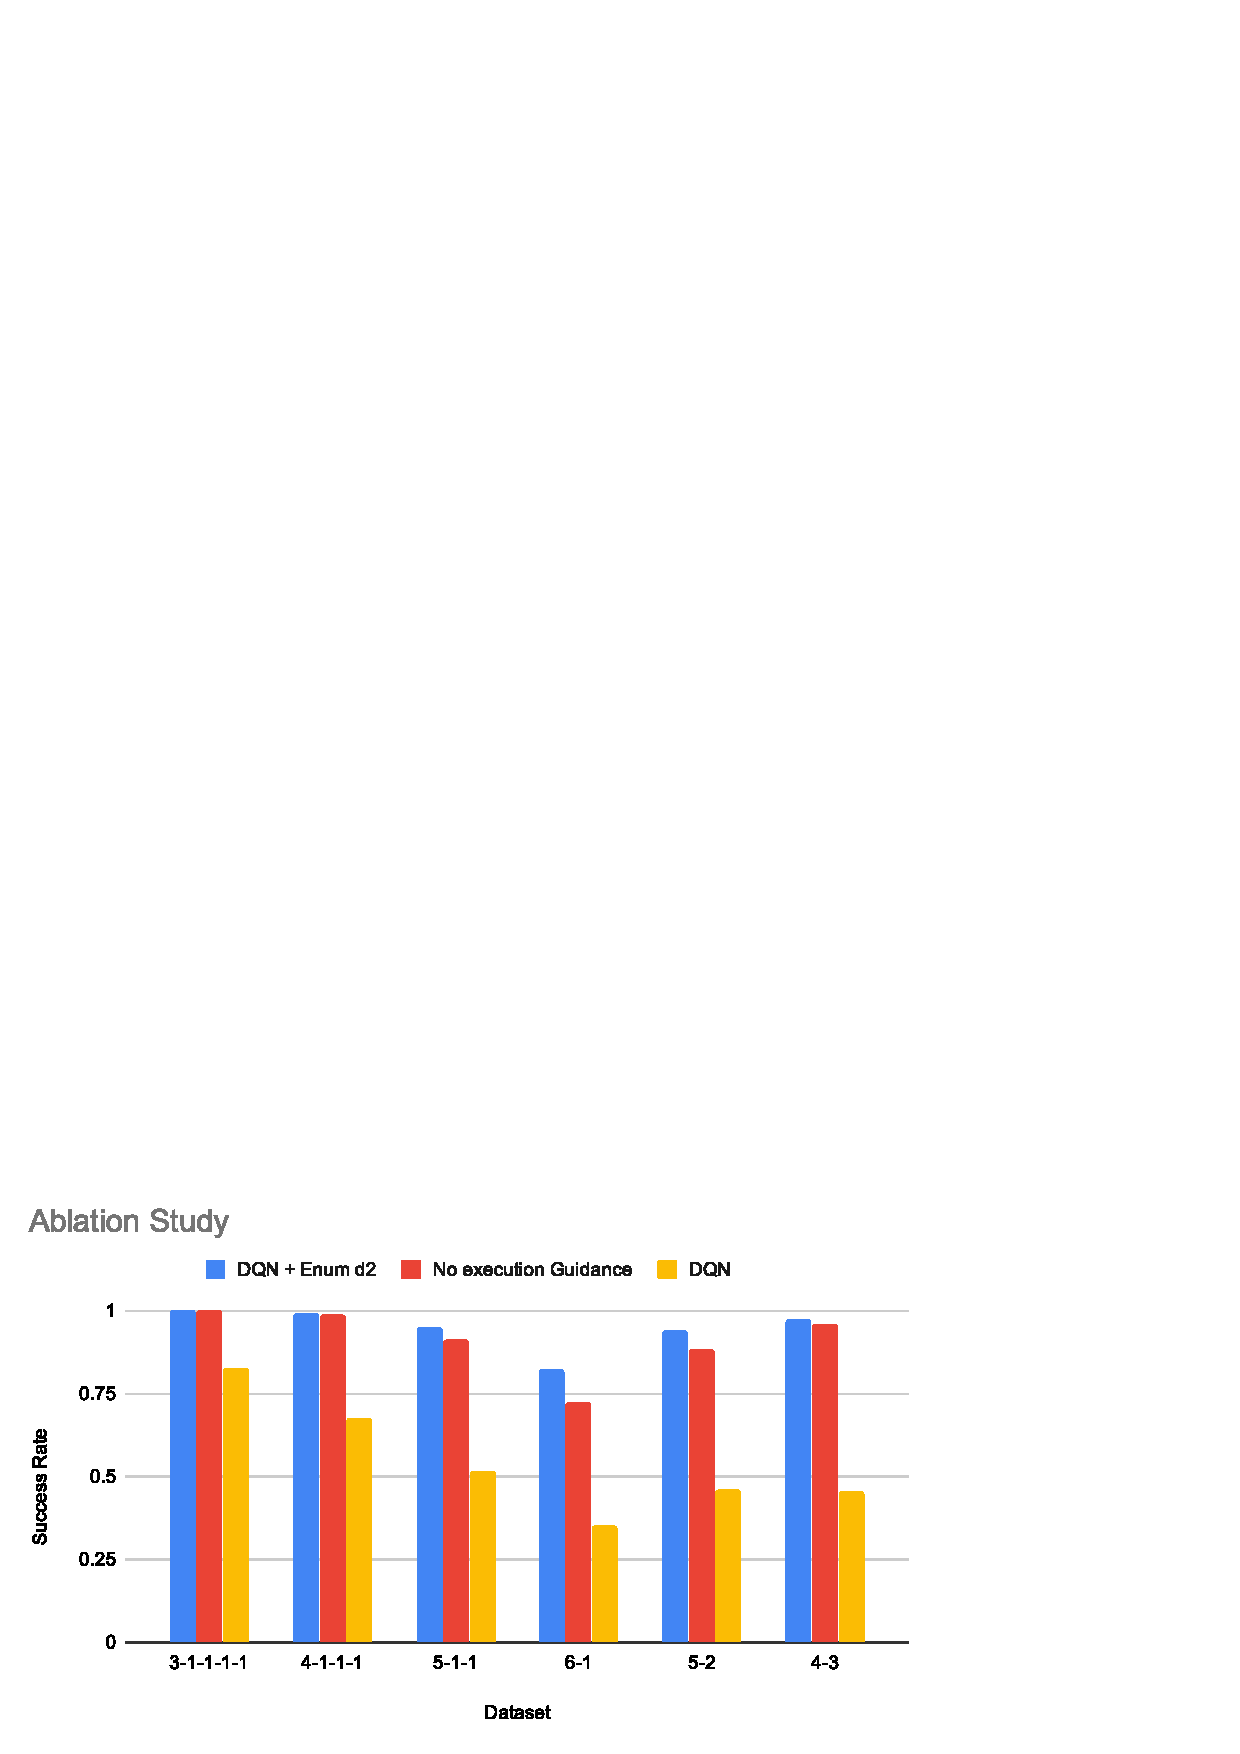
\includegraphics[width=0.4\textwidth]{ablations.pdf}
\caption{Fraction of problem instances solved in a variety of benchmarks by different algorithms. Left: Comparing our algorithm (black) to baselines neurosymbolic synthesis (blue) and enumerative synthesis with $M=3$ (red). Right: Comparing our algorithm (black) to ablations without hierarchical synthesis (green) and without execution guidance (yellow).} %\aws{would be nice to have a legend---it's atypical to have colors in only in caption}
\label{fig:baselines}
\end{figure*}

%We first discuss the datasets we evaluate on. Followed with the comparison of the implementation details between our model and baselines, and then we show an ablation study on the performance, generalizability, and robustness across the models. 

We evaluate our approach on the CLEVR dataset, both (i) on purely synthetic graphs that we generated, and (ii) on graphs constructed using a CNN based on the synthetic images in the dataset. As we discuss below, we focus on synthetic data since it allows us to generate challenging problem instances that require the use of relationships involving multiple objects (in this case, spatial relationships). Based on these datasets, we demonstrate that our approach outperforms several baselines and ablations.

\subsection{Experimental Setup}

\textbf{Synthetic graphs.}
%
The first dataset is a set of synthetic scene graphs that include objects and relations between these objects, including unary ones (called \emph{attributes}), namely shape, color, and material, as well as binary ones that encode spatial relations, namely front/behind and left/right.

Using this approach, we can create challenging problem instances (i.e., a scene graph and a target object) to evaluate our algorithm. Our primary goal is to create problem instances where the referring relational program has to include spatial relationships to identify the target object. These instances are challenging since multiple relations are needed to distinguish two identical objects---e.g., in Figure~\ref{fig:example} (left), at least two relations are needed to distinguish G from H, and more are needed in Figure~\ref{fig:example} (right).

To this end, we create graphs with multiple identical objects in the scene. We classify these datasets by the set of counts of identical objects (in terms of attributes). For instance, the dataset CLEVR-4-3 consists of 7 objects total, the first 4 and last 3 of which have identical attributes---e.g., it might contain 4 gray metal cubes and 3 red metal spheres.

For simplicity, we directly generate scene graphs; thus, they do not contain any uncertainty. We impose constraints on the graphs to ensure they can be rendered into actual CLEVR images if desired. We consider the following datasets: 3-1-1-1-1, 4-1-1-1, 5-1-1, 6-1, 5-2, and 4-3. For each dataset, we use 7 total objects. Each dataset has 30 scene graphs for training (a total of 210 problem instances), and 500 scene graphs for testing (a total of 3500 problem instances).

\textbf{CLEVR images.}
%
We also evaluate based on a dataset of images from the original CEVR dataset. These images have the same kinds of relations as our generated scene graphs.

We use a convolutional neural network (CNN) to construct the scene graph~\cite{yi2018neural}. For simplicity, this CNN predicts both object attributes and positions. The object attributes are predicted independently---i.e., it could predict that object J is both red with probability $0.75$ and purple with probability $0.75$. We consider a relation to be absent if $p=p(\rho(o_1,...,o_n))<1/2$; for relations with $p\ge1/2$, we consider them to be uncertain if there are multiple such attributes of the type (e.g., object J is predicted to be both red and purple with probability $\ge1/2$), and certain otherwise. The spatial relationships are inferred based on the object positions; we consider it to be uncertain if the objects are very close together along some dimension.

\textbf{Our algorithm.}
%
We search for programs of length at most $M=8$, using $K=2$ in hierarchical synthesis. We consider three variables---i.e., $|\mathcal{Z}|=3$, including $\tvar$. We use $N=200$ rollouts during reinforcement learning. We pretrain our $Q$-network on the training set corresponding to each dataset, using $N=10000$ gradient steps with a batch size of $5$.

\subsection{Comparison to Baselines}

We use each algorithm on our synthetic graphs dataset; in Figure~\ref{fig:baselines} (left), we report what fraction of each kind of problem instance that is solved by each one.

\textbf{Neurosymbolic synthesis.}
%
We compare to a state-of-the-art synthesizer called Metal~\cite{si2018learning}. This approach uses reinforcement learning to find a program that satisfies the given specification; in addition, they use the same simple meta-learning approach as ours. As can be seen in Figure~\ref{fig:baselines}, our approach substantially outperforms this baseline by using hierarchical synthesis and execution-guided synthesis. For instance, on 6-1, our approach solves 82\%; in contrast, Metal solves just 19\%. Similarly, on 4-3, our approach solves 97\% whereas Metal solves just 6\%. We believe Metal works poorly in our setting due to the lack of intermediate feedback in our setting.

\textbf{Enumerative synthesis.}
%
We compare to a synthesis algorithm that enumerates programs to find one that solves the task~\cite{alur2013syntax}. This approach does not use machine learning to guide its search, making it challenging to scale to large programs (i.e., large $M$) due to the combinatorial blowup in the search space; thus, we consider $M=3$. As can be seen in Figure~\ref{fig:baselines}, our approach substantially outperforms enumerative synthesis. For instance, on 6-1, our approach solves 82\%, whereas enumerative synthesis solves 42\%, and on 4-3, our approach solves 97\%, whereas enumerative synthesis solves 41\%.

%\textbf{Greedy algorithm.}
%
%Finally, we compare to an algorithm that greedily selects the most promising relations to include based on how many assignments $\tvar\to o$ they remove, where $o$ is an object in $G$. Intuitively, this approach performs best when attributes are sufficient to distinguish the target object, since in this case reasoning about multiple relations is unnecessary. As can be seen in Figure~\ref{fig:baselines}, our algorithm substantially outperforms this approach, especially on the more challenging problem instances.

\subsection{Comparison to Ablations}

We compare to two ablations on the synthetic graph datasets; in Figure~\ref{fig:baselines} (right), we report what fraction of the benchmarks in each category are solved.

\textbf{Hierarchical synthesis.}
%
Next, we compare to an ablation that does not use hierarchical synthesis---i.e., it only count the program generated by the neural symbolic synthesizer, but no enumerative search to correct the generated program. As can be seen, our approach substantially outperforms this ablation---e.g., on 6-1, hierarchical synthesis improves performance from 35\% to 82\%, and on 4-3, it improves performance from 46\% to 97\%. Intuitively, hierarchical synthesis improves performance by using reinforcement learning to find the larger but more straightforward parts of the program, whereas the enumerative synthesizer can find the more challenging parts using brute force.

\textbf{Execution guidance.}
%
We compare to an ablation where we do not use the interpreter to guide RL; instead, the states are partial programs $P$. In particular, this ablation does not have feedback from the interpreter until the sparse reward at the very end of a rollout. As can be seen from Figure~\ref{fig:baselines}, using execution guidance improves our performance, especially on harder benchmarks---e.g., for the 6-1 benchmark, it improves performance from 72\% to 82\%.

\subsection{CLEVR Images}

We tested our approach on CLEVR images where we constructed the scene graph using a CNN~\cite{yi2018neural}. Out of 6487 tasks, our approach solved all but 25 according to the ground truth relations---i.e., the ground truth in the CLEVR dataset, not the predicted ones seen by our interpreter. Thus, our approach works well even when there is uncertainty in the scene graph predicted using a CNN.

%Other than the DQN model, we have explored quite a few different models, encoding and decoding strategies. We evaluate the performance on a handcrafted unit test, with one scene and 3 objects. We define passing the unit test as the model can overfit to the dataset in 10000 gradient steps. 

%The GNN converts a graph into a matrix of node representations. The common practice utilizing the latent matrix is to combine them to one single global representation and decode from the latent vector. We propose a different strategy called local action decoding. We select the corresponding nodes which have a direct impact on the action along with the global representation and pass these embeddings through a neural network to obtain scores for the exact action. Then we pick the corresponding action based on the scores. 
%$s = \pi mask(M)$
%\begin{align*}
%s &= \pi_{\theta} \textit {mask} (M)
%\end{align*}

%We evaluate the performance of a unit test scene with three objects. We compare the performance based on the training error. If the model cannot overfit to the simple unit test, it means the model cannot learn well. 

%Utilizing the local action decoding strategy better captures the local information than utilizing the global representation alone. We compared the performance over three different ways to obtain the global embedding and the local action decoding method under the policy gradient reinforcement learning algorithm. The global embeddings are obtained by aggregation, attention layer, and add a global node in the graph. Regardless of how the global embedding is generated, we found that only the local action decoding strategy passes the unit test.

%By adding the interpreter in the learning loop, we can provide further execution guidance to the learning process: rather than obtaining the reward only at the end of rollouts, we have intermediate reward for each clause taken; the states are unified for partial programs with the same effects but different expressions; we also have a wider range of reinforcement learning algorithm to choose from, as Q-learning algorithms requires separable states.

%We compare the performance of the models by the success rate. In terms of the gradient-based methods, our method significantly outperforms the LSTM baseline, especially when the test dataset difficulty increases. Although the enumerative method performs well in terms of accuracy, it has an exponential time complexity and query number as the depth grows. Therefore, we use the enumerative method to evaluate the difficulty of the dataset and the capability of the neural network models. 

%We consider the enumerative approach as the most general method and use the enumerative approach to denote the difficulty of the datasets. For the DQN method, the accuracy falls mostly in the Enum-d3 range, while the LSTM method is approximately Enum-d2. By further comparing the DQN + Enum 1 and LSTM + Enum 1, our method also demonstrates better generalizability on the harder datasets. 

%\subsection{Optimization}
%\subsection{Dataset}

\section{Conclusions}

We have proposed an approach to solving a symbolic variant of referring expressions using program synthesis. Our work is a first step towards incorporating symbolic reasoning into image captioning tasks. Future work includes leveraging our approach to generate natural language referring expressions for real-world images---i.e., by synthesizing a referring relational program and translating it to natural language. In addition, we have ignored the problem of \emph{naturalness} for the programs we generate (i.e., how easy it is for a human to understand the program), since we are focused on cases where complex logical reasoning is needed; in practice, naturalness is an important criterion that must be addressed.